\documentclass[aspectratio=1610,polish]{beamer} %If you want to create Polish presentation, replace 'english' with 'polish' and uncomment 3-th line, i.e., '\usepackage{polski}'
\usepackage[utf8]{inputenc} %Only needed fot pdflatex
\usepackage[T1]{fontenc}
\usepackage{indentfirst}
\usepackage[english,polish]{babel}
\usepackage{polski}
\frenchspacing

\usepackage{listings} %We want to put listings
\usepackage[binary-units]{siunitx}
\sisetup{output-decimal-marker = {,}}
\usepackage{icomma}
\usepackage{pgfplots}
\pgfplotsset{compat=1.15}
\usepackage{csquotes}
\DeclareQuoteAlias{croatian}{polish}

\AtBeginDocument{
  \renewcommand{\tablename}{Tablica}
  \renewcommand{\figurename}{Rysunek}
}

\usepackage{import}
\usepackage{dirtree}

\usepackage[%
style=numeric,
sorting=none,
language=autobib,
autolang=other,
backend=biber,
]{biblatex}

\addbibresource{../artykul/bibliografia.bib}

\mode<beamer>{ 	%in 'beamer' mode
  \hypersetup{pdfpagemode=FullScreen}		%Enable Full screen mode
  \usetheme[parttitle=rightfooter]{AGH}		%Show part title in right footer
  %\usetheme[nosidebar]{AGH}			%Do not show sidebar on non-title slides
  %\usetheme[nosidebar,margins=1em]{AGH}		%Do not show sidebar on non-title slidesa and set both margins (left / right) to 1em
  %\usetheme[dark]{AGH}                 		%Use dark background
  %\usetheme[dark,parttitle=leftfooter]{AGH}  	%Use dark background and show part title in left footer
}
\mode<handout>{	%in 'handout' mode
  \hypersetup{pdfpagemode=None}		
  \usepackage{pgfpages}
  \pgfpagesuselayout{4 on 1}[a4paper,border shrink=5mm,landscape]	%show 4 slides on 1 page
  \usetheme{boxes}
  \addheadbox{structure}{\quad\insertpart\hfill\insertsection\hfill\insertsubsection\qquad} 	%content of header
  \addfootbox{structure}{\quad\insertauthor\hfill\insertframenumber\hfill\insertsubtitle\qquad} 	%content of footer
}

\AtBeginPart{ %At begin part: display its name
  \frame{\partpage}
} 

\title[Wibroakustyczna stacja pomiarowa]{%
Wibroakustyczna stacja pomiarowa oparta o mikrokomputer Raspberry Pi}
\author[S. Mikulicz, M. Piszak]{Szymon Mikulicz\\Marcel Piszak}
\date{2018-04-13}
\institute[AGH]{%
  Koło Naukowe Informatyki w Wibroakustyce\\
  ,,LabAcoustics''\\
  \url{http://www.labacoustics.agh.edu.pl}\\
  Opiekun: dr inż. Paweł Pawlik
}
%%%%%%%%%%% Configuration of the listings package %%%%%%%%%%%%%%%%%%%%%%%%%%
% Source: https://en.wikibooks.org/wiki/LaTeX/Source_Code_Listings#Using_the_listings_package
%%%%%%%%%%%%%%%%%%%%%%%%%%%%%%%%%%%%%%%%%%%%%%%%%%%%%%%%%%%%%%%%%%%%%%%%%%%%
\lstset{ %
  backgroundcolor=\color{white},   % choose the background color
  basicstyle=\footnotesize,        % the size of the fonts that are used for the code
  breakatwhitespace=false,         % sets if automatic breaks should only happen at whitespace
  breaklines=true,                 % sets automatic line breaking
  captionpos=b,                    % sets the caption-position to bottom
  commentstyle=\color{green},      % comment style
  deletekeywords={...},            % if you want to delete keywords from the given language
  escapeinside={\%*}{*)},          % if you want to add LaTeX within your code
  extendedchars=true,              % lets you use non-ASCII characters; for 8-bits encodings only, does not work with UTF-8
  frame=single,	                   % adds a frame around the code
  keepspaces=true,                 % keeps spaces in text, useful for keeping indentation of code (possibly needs columns=flexible)
  keywordstyle=\color{blue},       % keyword style
  morekeywords={*,...},            % if you want to add more keywords to the set
  numbers=left,                    % where to put the line-numbers; possible values are (none, left, right)
  numbersep=5pt,                   % how far the line-numbers are from the code
  numberstyle=\tiny\color{gray},   % the style that is used for the line-numbers
  rulecolor=\color{black},         % if not set, the frame-color may be changed on line-breaks within not-black text (e.g. comments (green here))
  showspaces=false,                % show spaces everywhere adding particular underscores; it overrides 'showstringspaces'
  showstringspaces=false,          % underline spaces within strings only
  showtabs=false,                  % show tabs within strings adding particular underscores
  stepnumber=1,                    % the step between two line-numbers. If it's 1, each line will be numbered
  stringstyle=\color{cyan},        % string literal style
  tabsize=2,	                   % sets default tabsize to 2 spaces
  title=\lstname,                  % show the filename of files included with \lstinputlisting; also try caption instead of title
  % needed if you want to use UTF-8 Polish chars
  literate={ą}{{\k{a}}}1
  {Ą}{{\k{A}}}1
  {ę}{{\k{e}}}1
  {Ę}{{\k{E}}}1
  {ó}{{\'o}}1
  {Ó}{{\'O}}1
  {ś}{{\'s}}1
  {Ś}{{\'S}}1
  {ł}{{\l{}}}1
  {Ł}{{\L{}}}1
  {ż}{{\.z}}1
  {Ż}{{\.Z}}1
  {ź}{{\'z}}1
  {Ź}{{\'Z}}1
  {ć}{{\'c}}1
  {Ć}{{\'C}}1
  {ń}{{\'n}}1
  {Ń}{{\'N}}1
}
%%%%%%%%%%%%%%%%%
\begin{document}
  \maketitle
  %%%%%%%%%%%%%%%%
  \section{Informacje wstępne}
  \begin{frame}{Wibroakustyczna systemy pomiarowe}
    \centering
    \begin{columns}
      \column{0.45\textwidth}
      Podejście klasyczne:
      \begin{itemize}
	\item Analogowy akcelerometr pomiarowy uznanej firmy (np. PCB)
	\item Karta pomiarowa z niskoszumowym przetwornikiem A/C
	\item Komputer z oprogramowaniem producenta do odczytu i zapisu danych
      \end{itemize}
      \column{0.45\textwidth}
      Podejście proponowane:
      \begin{itemize}
	\item Cyfrowy moduł z akcelerometrem typu MEMS oraz przetwornikiem A/C
	\item Komputer Raspberry Pi z otwartym oprogramowaniem dostosowanym do
	  odczytu i zapisu danych
      \end{itemize}
    \end{columns}
  \end{frame}
  %%%%%%%%%%%%%%%%
  \begin{frame}{Założenia projektowe}
    \begin{itemize}
      \item Pomiary zgodne z normą PN-B 02170:2016-12
      \item Pasmo częstotliwości od \SI{0.5}{\hertz} do \SI{100}{\hertz}
      \item Amplituda przyspieszenia drgań od
	\SI{e-3}{\metre\per\square\second} do \SI{10}{\metre\per\square\second}
      \item Możliwość zapisu w pamięci urządzenia zarejestrowanych wibrogramów
    \end{itemize}
  \end{frame}
  %%%%%%%%%%%%%%%%
  \section{Realizacja}
  \begin{frame}{Konstrukcja stacji pomiarowej}
    \begin{columns}
      \column{0.4\textwidth}
      \begin{itemize}
	\item Raspberry Pi 3 model B
	\item Karta pamięci microSD 16GB
	\item Moduł akcelerometru MEMS Adafruit MMA8451
	\item Kable połączeniowe
	\item Zasilacz
      \end{itemize}
      \column{0.59\textwidth}
      \begin{figure}
	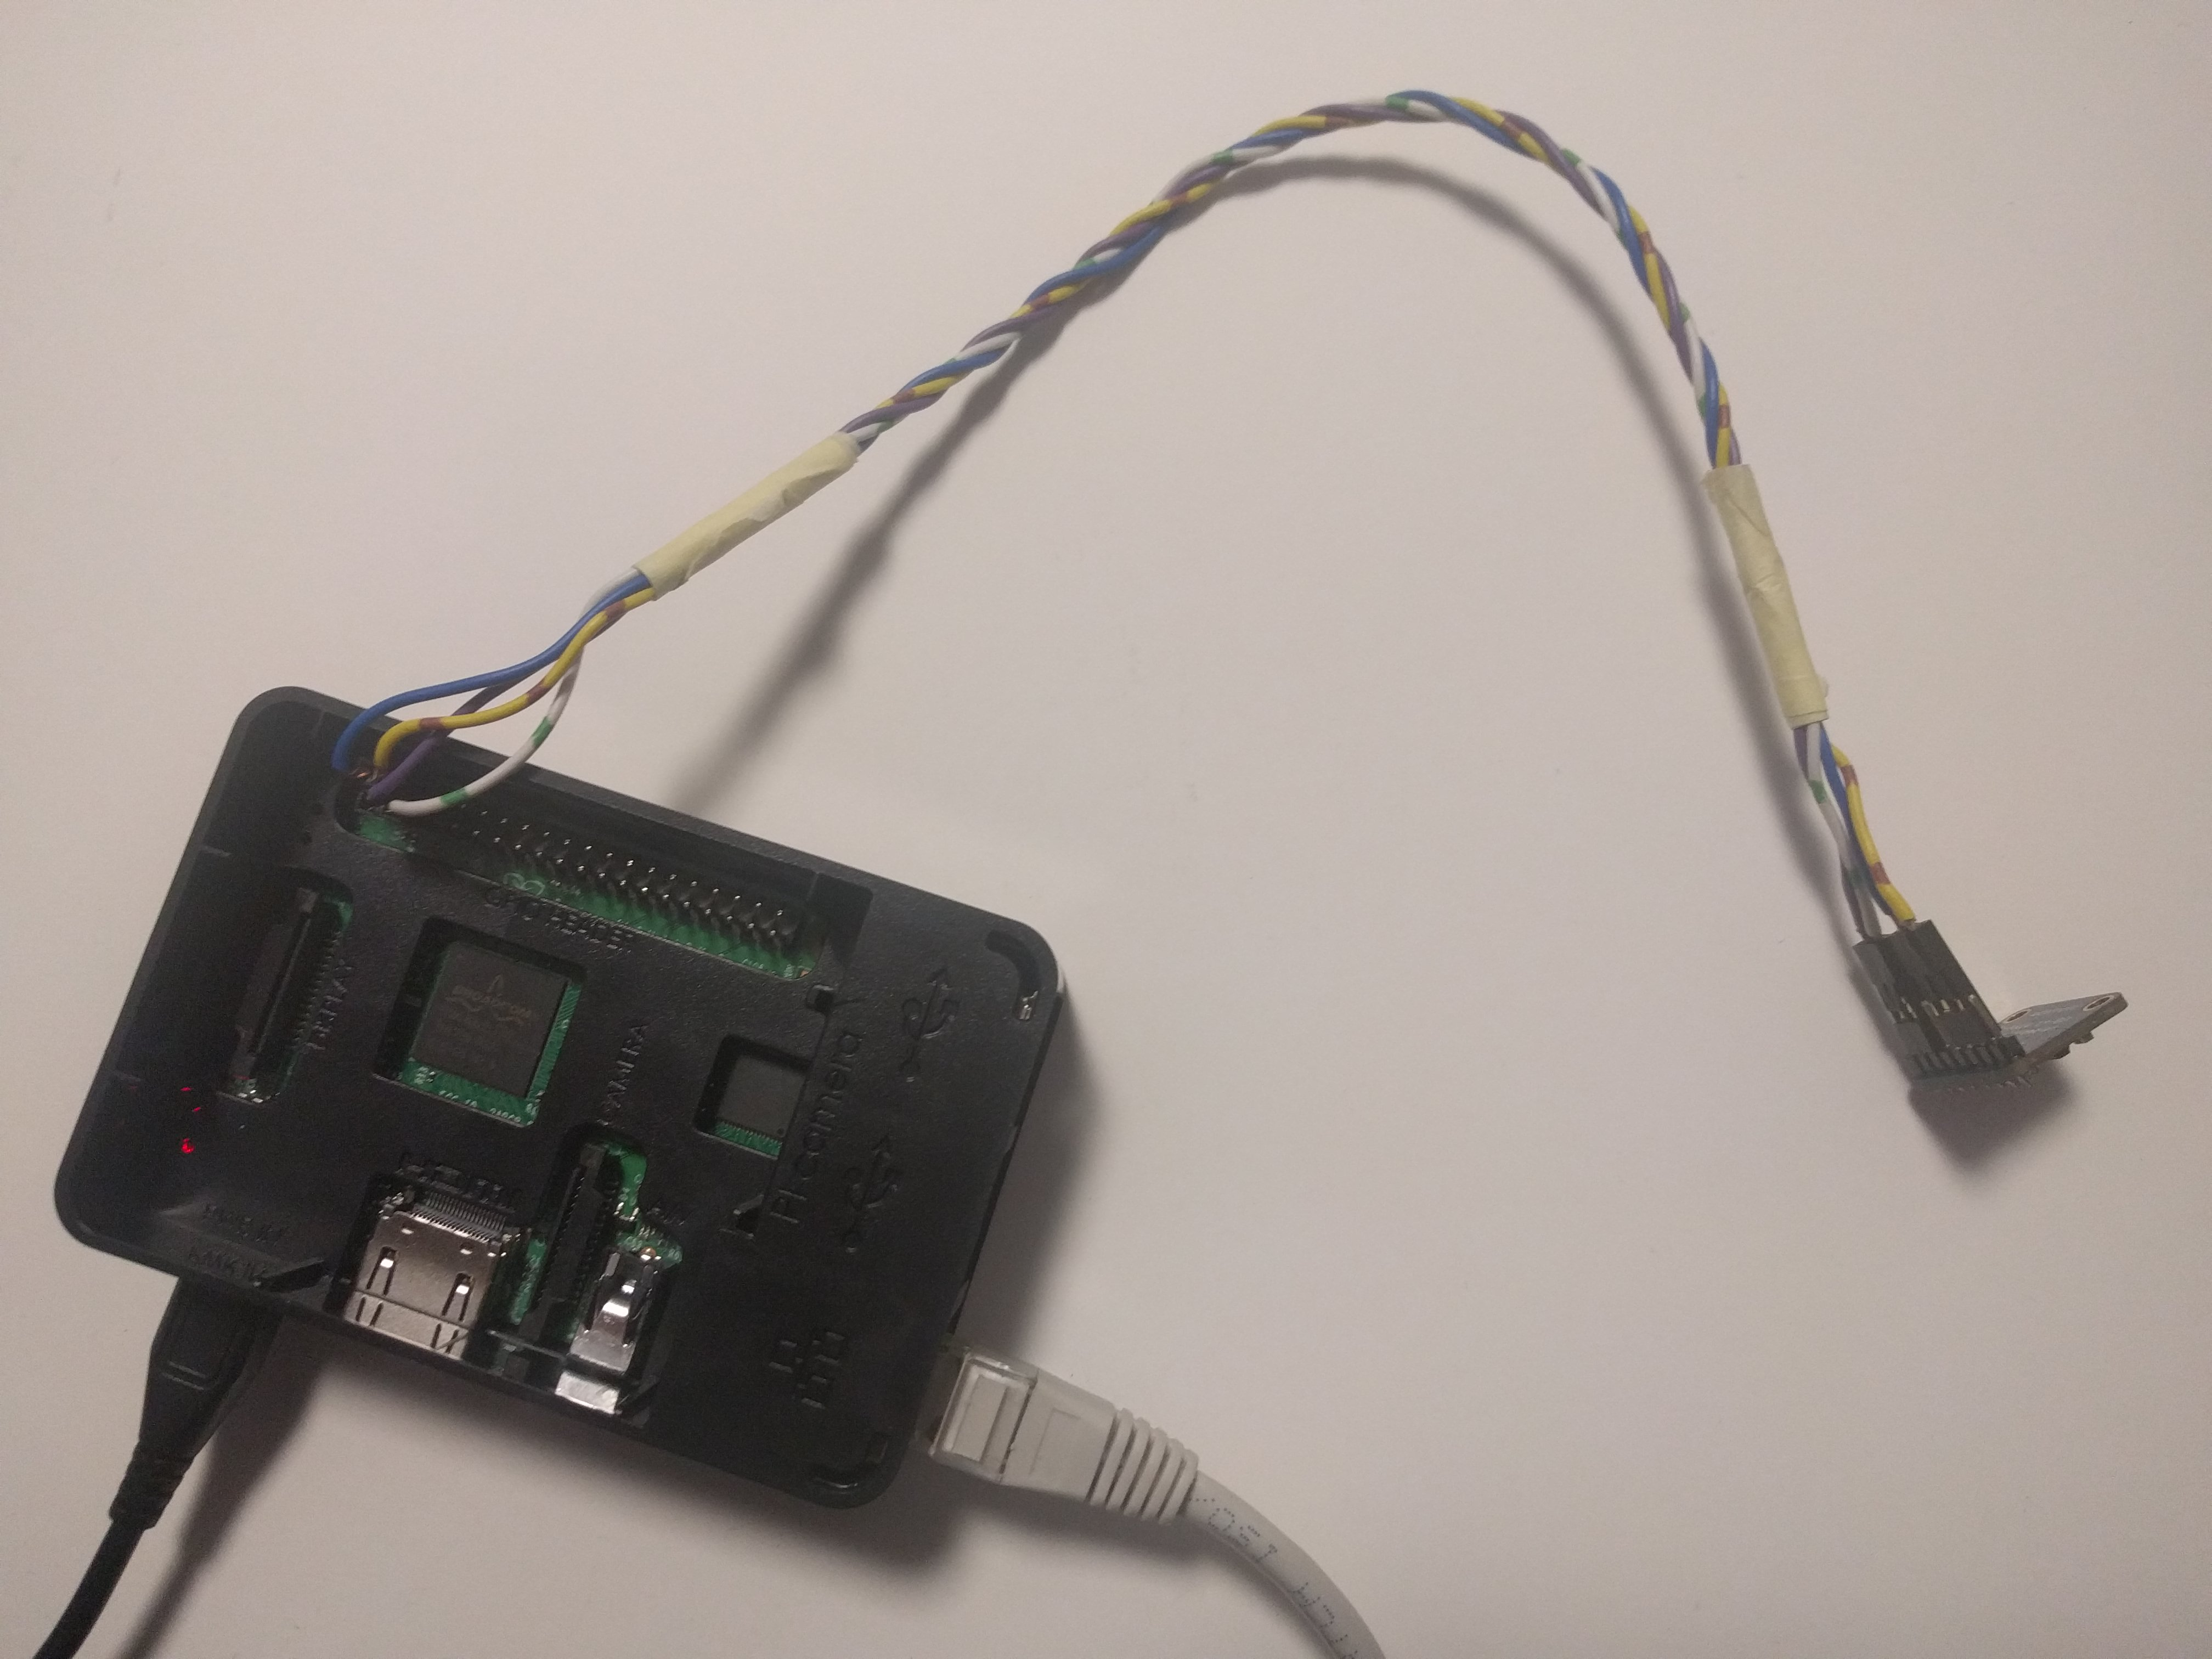
\includegraphics[width=\textwidth]{../artykul/bitgraphics/pi.png}
	\caption{Prototyp stacji pomiarowej}
      \end{figure}
    \end{columns}
  \end{frame}
  %%%%%%%%%%%%%%%%
  \begin{frame}{Komunikacja z modułem i jego ustawienia}
    \begin{columns}
      \column{0.4\textwidth}
      \begin{itemize}
	\item Protokół transmisji danych -- I\textsuperscript{2}C (SDA -- dane,
	  SCL -- zegar)
	\item Częstotliwość próbkowania -- \SI{800}{\hertz}
  \item Zakres pomiarowy -- $\pm\SI{2}{\g}$
  \item Rozdzielczość bitowa -- \SI{14}{\bit}
      \end{itemize}
      \column{0.59\textwidth}
      \begin{figure}
	\import{vecgraphics/}{schemat.pdf_tex}
	\caption{Schemat stacji pomiarowej}
      \end{figure}
    \end{columns}
  \end{frame}
  %%%%%%%%%%%%%%%%
  \begin{frame}{Opis programu sterującego}
    \begin{columns}
      \column{0.59\textwidth}
      \begin{itemize}
        \item Komunikacja z urządzeniem poprzez odczyt z i zapis do rejestrów
        \item Wykorzystanie wewnętrznej kolejki FIFO akcelerometru (\SI{32}{\bit})
        \item Wysyłka sygnału przerwania w momencie zapełnienia połowy kolejki
        \item Akumulacja wyników z wybranego okresu
        \item Zapis wibrogramu do pliku HDF5
      \end{itemize}
      \column{0.4\textwidth}
      \begin{figure}
      \begin{minipage}{\textwidth}
      \dirtree{%
      .1 <rok>/.
      .2 <miesiąc>/.
      .3 <dzień>/.
      .4 <godzina>/.
      .5 <minuta>.
      .5 \dots.
      .4 \dots.
      .3 \dots.
      .2 \dots.
      }%
      \end{minipage}
      \caption{Struktura pliku z wynikami}
      \end{figure}
    \end{columns}
  \end{frame}
  %%%%%%%%%%%%%%%%
  \begin{frame}[fragile]{Fragment kodu}
    \begin{lstlisting}[language=Python]
      from mma8451.register import register as REG
      from mma8451.iic import IIC
      import pigpio
  
      # Inicjalizacja połączenia z procesem pigpio
      pi = pigpio.pi()
      # Stwórz obiekt klasy, gdzie 1 do magistrala a 0x1D adres
      iic = IIC(pi, 1, 0x1D)
      # Uśpij urządzenie
      iic.unset_flag(REG.CTRL_REG1.ACTIVE)
      # Włącz tryb 14-to bitowy
      iic.unset_flag(REG.CTRL_REG1.F_READ)
      # Włacz urządzenie do trybu aktywnego
      iic.set_flag(REG.CTRL_REG1.ACTIVE)
      # Pobierz dane ze wszystkich trzech osi
      dane = iic.block_read(REG.OUT_X_MSB, 6)\end{lstlisting}
  \end{frame}
  %%%%%%%%%%%%%%%%
  \begin{frame}{Przeprowadzone testy}
    \begin{columns}
      \column{0.48\textwidth}
      \begin{figure}
        \includegraphics[width=\textwidth]{bitgraphics/stacja_2.png}
        \caption{Wyznaczanie charakterystyki}
      \end{figure}
      \column{0.48\textwidth}
      \begin{figure}
        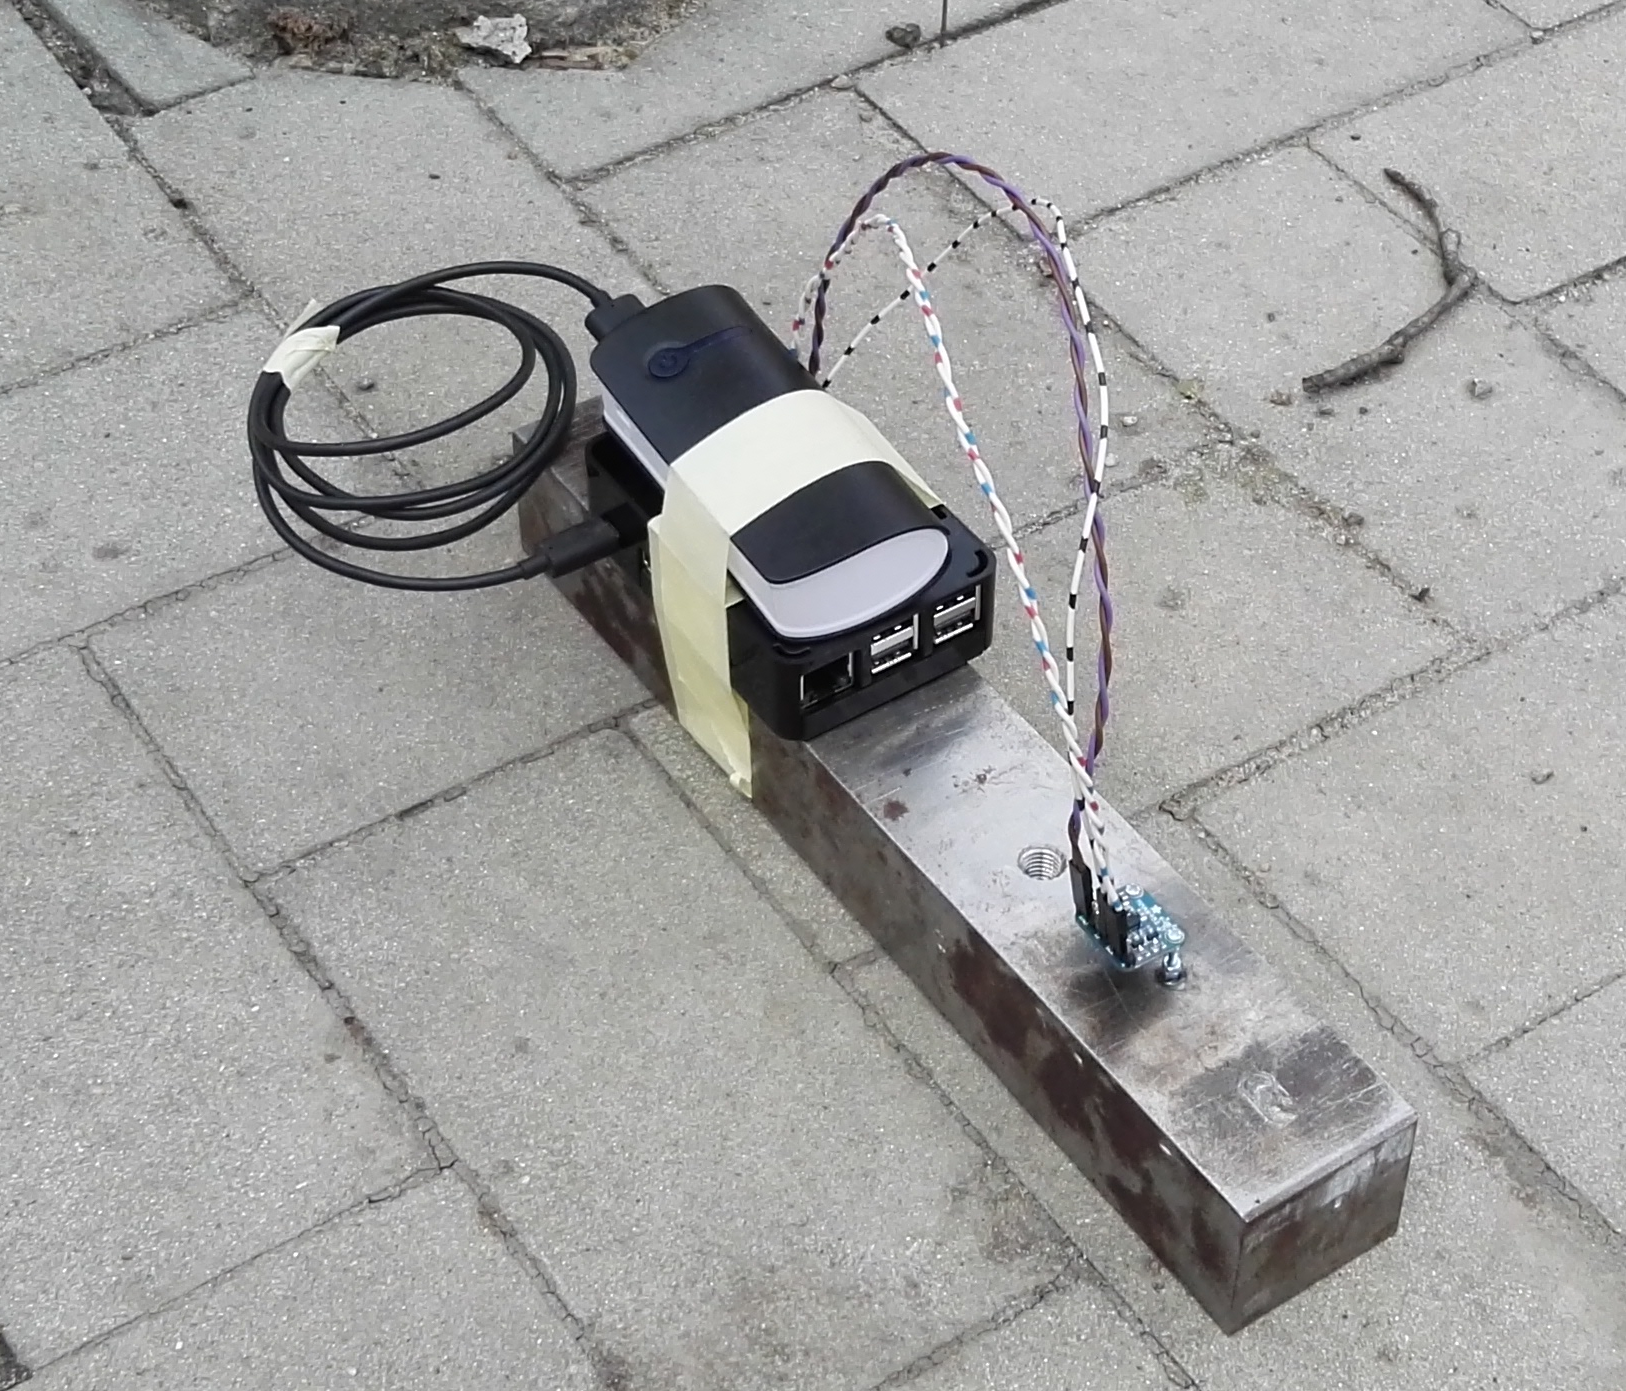
\includegraphics[width=\textwidth]{bitgraphics/stacja_1.png}
        \caption{Pomiar kontrolny}
      \end{figure}
    \end{columns}
  \end{frame}
  %%%%%%%%%%%%%%%%
  \section{Wyniki}
  \begin{frame}{Charakterystyka akcelerometru}
    \begin{figure}
      \input{plots/char.pgf}
    \end{figure}
  \end{frame}
  %%%%%%%%%%%%%%%%
  \begin{frame}{Wibrogram przejeżdżających tramwajów}
    \begin{figure}
      \input{plots/ul_maj.pgf}
    \end{figure}
  \end{frame}
  %%%%%%%%%%%%%%%%
  \section{Podsumowanie}
  \begin{frame}{Podsumowanie realizacji}
    \begin{itemize}
      \item Na podstawie danych zarejestrowanych przez stację można określić w której strefie zagrożenia znajduje się budynek
      \item W zakresie pomiarowych charakterystyka akcelerometru jest porównywalna z rozwiązaniami komercyjnymi
      \item Mały odstęp sygnału od szumu urządzenia ogranicza jego zastosowania
    \end{itemize}
  \end{frame}
  %%%%%%%%%%%%%%%%
  \begin{frame}{Dalsze prace}
    \begin{columns}
      \column{0.4\textwidth}
      \begin{itemize}
        \item Zastosowanie dokładniejszych akcelerometrów
        \item Rozszerzenie stacji o funkcjonalność pomiaru hałasu (mikrofony MEMS)
        \item Rozszerzenie oprogramowania o funkcjonalność sieciową
        \item Połączenie wielu stacji pomiarowych w rozproszony system korzystający z technologii IoT
      \end{itemize}
      \column{0.59\textwidth}
      Tu znajdze się zdjęcie akcelerometru z obudową
    \end{columns} 
  \end{frame}
  %%%%%%%%%%%%%%%%
  \begin{frame}{Bibliografia}
    \nocite{*}
    \printbibliography
  \end{frame}
  %%%%%%%%%%%%%%%%
  \begin{frame}
    \centering
    \vspace*{40pt}

    {\huge Dziękujemy za uwagę}
    \vspace*{20pt}

    Projekt dostępny pod adresem:\\
    \url{https://github.com/Ashymad/OSKA-Pi-MEMS}
    \url{https://github.com/Ashymad/python-mma8451}
  \end{frame}
\end{document}

